\chapter{Methodology}
\label{chapter:method}

\section{Overview}
The two main core objectives of our work involve in producing an online multi object tracker, which incorporates the spatiotemporal coherence of object motion together with the appearance consistency and producing a panoptic segmentation of the video feed by taking into account the bipartite potentials.

\section{Multi Object Tracker}

In this section, we describe our approach for online real-time multi-object tracking. The core of our work surrounds three key attributes; an LSTM network tackling track position estimates as a probabilistic classification problem, a methodology for similarity extraction and track association that is aware of occlusions, crossovers, and other identified key challenges and finally, the extension of track predictability to the BEV space exploiting its properties. Further, we explore the possibility of propagating input uncertainties through the LSTM network. The naive integration of a generic LSTM network to exploit the temporal aspect overlooks some key aspects of the problem including uncertainty of detection positions and requirement for estimating a possible region of object presence. To address this work, we introduce an LSTM network with probabilistic outputs also capable of capturing the input uncertainties. Our final model shown in \ref{fig:tracker} performs on-par with current state-of-the-art object trackers and operates in real-time. Our model is tested on popular tracking datasets, MOT16 \cite{DeepSiam:MilanL0RS16} and KITTI-tracking \cite{DeepSiam:KITTI}. These two datasets are from slightly different domains (the former focuses on general indoor and outdoor scenes while the latter contains videos of roads taken from the perspective of a vehicle). This allows us to verify that our work solves a generalized tracking problem as opposed to a single-domain specific solution or being optimized onto a single dataset. Our work is explained under six subsections. The LSTM network along with our unique contribution is outlined initially. Then we lay out the appearance similarity usage in a multi-object domain followed by the track association problem and overall 2D tracker. Finally, we explain the extensibility of our LSTM model for accurate 3D track prediction and the improvements gained from BEV space constraints.


\subsection{LSTM network}

\begin{figure*}[t]
	\centering
	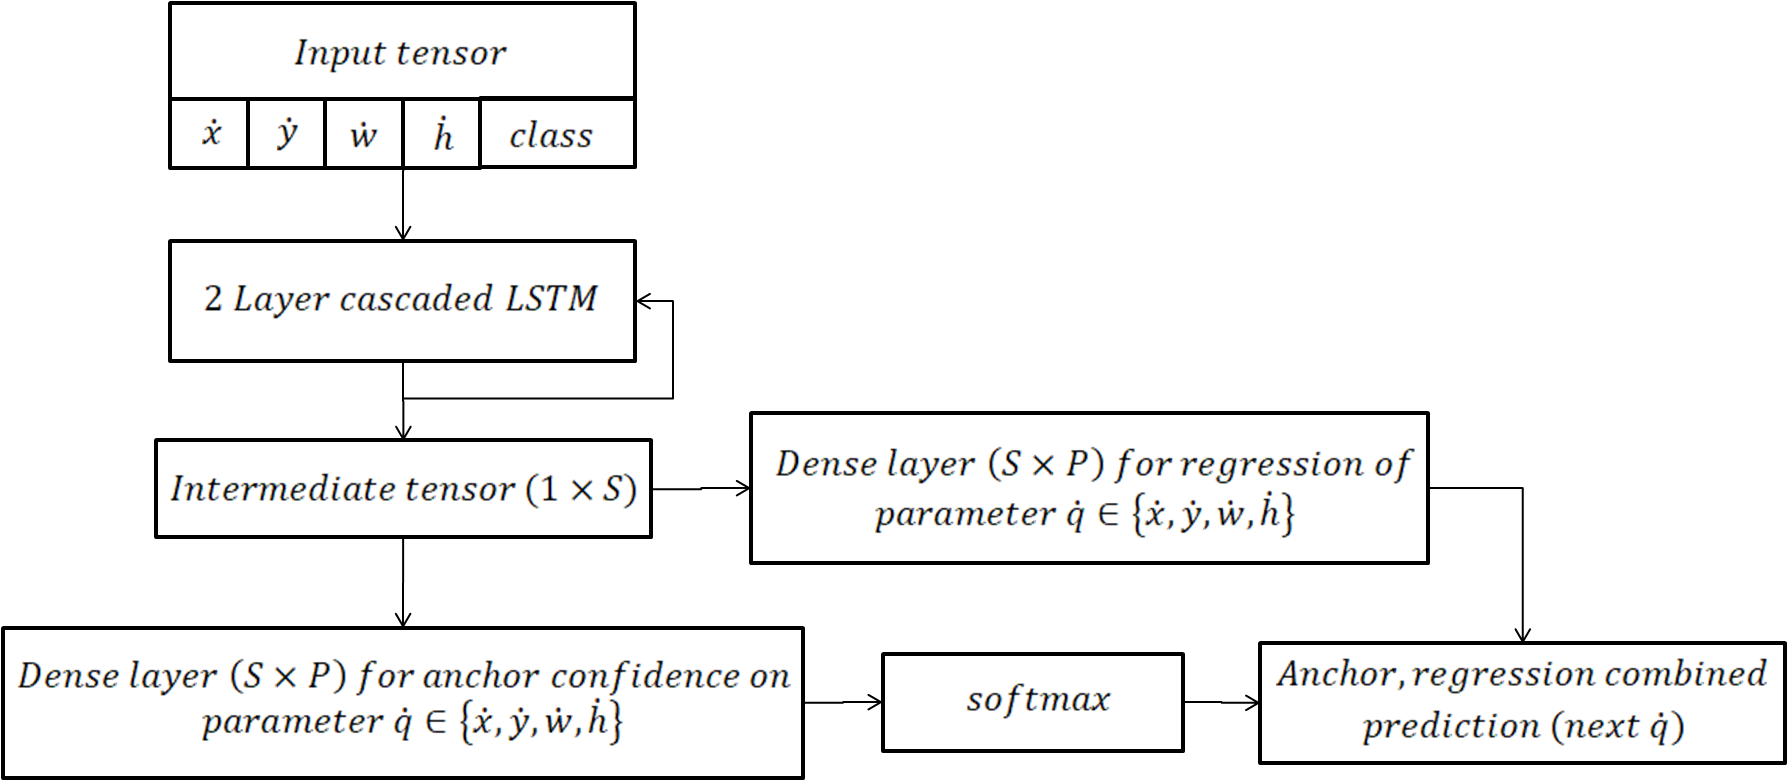
\includegraphics[ width=\textwidth]{figs/LSTM_network.png}
	\vspace{-0.5cm}
	\caption{Structure of the proposed LSTM network}
	\label{fig:LSTM_network}
	\vspace{0.5cm}
\end{figure*}

Consider a video as a sequence of image frames i.e. $V = I_{0},I_{1},...,I_{n}$ where $I_{k}$ s a matrix of fixed dimensions. Given detections $D = D_{0},D_{1},...,D_{n}$, for the objects present in each frame , where each  is a list of bounding box locations, class predictions, and other information corresponding to objects contained in the image , our goal here is to estimate the bounding box co-ordinates $B_{k,i}$ for each object in the following frame; $I_{k+1}$. Note that  $B_{k,i} = (x_{k,i},y_{k,i},h_{k,i},w_{k,i})$ where $x,y,h,w$ correspond to $x,y$ co-ordinates of centre, height and width of the bounding box for the $i^{th}$ object in the $k^{th}$ frame. Further, this system would operate in an online setting where at any given instance when time $t = k$, the frames, hence detections too are present only up to $I_{k}$ and $D_{k}$ espectively. Further the $i^{th}$ object will be consistent across consecutive frames (obtained using the output of the system) until the object disappears. The LSTM component can be viewed as a function $L$ with $L(D_{0},D_{1},...,D_{k}) = F_{k}$ where $F_{k}$ is a list of temporally aware feature maps $F_{k,i}$ corresponding to each object $i$ present within $D_{k}$. The remaining two functions; $C$ and $R$ correspond to classification (selecting anchor) and regression (estimating deviation from anchor) of the exact bounding box targets. Each bounding box datum $(x,y,h,w)$ is interpreted as a deviation from the previous time step $(\dot{x},\dot{y},\dot{h},\dot{w})$ which reduces the mean of those variables. Note that due to the discrete nature of data, $\dot{x} = x - x_{i-1}$ Using normalized co-ordinates $(x,y,h,w)$ values divided by relevant image dimensions); this range will be within $(-1, 1)$ and an optimum number of anchors can be used to estimate this value as a classification problem. 
\par Having laid down the classifications on to the targets, the required estimates from the classification function would be a one hot encoded tensor; $C_{out}$ of shape $(P, 4)$ for $P$ bins of anchors and 4 bounding box parameters. In our work, we use four bins; 0, 0.1, 0.5, 0.8 leading to a $(4, 4)$ tensor where the bin closest to the target value (ex: $\dot{x}$)  on each row would contain one and the rest zero. Each selected bin is an anchor located at a specific distance away from the next expected value for the parameter considered. The classification function can be presented as $C(F_{k,i}) = C_{out}$ The regression function output would be a similarly shaped tensor $R_{out}$. It is essential for the loss function to consider the nature of both the classification as well as regression outputs of the network. The overall model of estimator is illustrated in \ref{fig:LSTM_network}. Here intermediate tensor corresponds to the temporally aware feature maps $F_{k,i}$ of the $i^{th}$ object and the system has four similar but separate instances of the dense layers to handle each parameter and that finally results in outputs $C_{out}$ and $R_{out}$. In essence the network estimates how far an object would move from its current position over the next time step. The $x,y$ components capture motion along the image axes while the $h,w$ components correspond to the motion along the depth axis as well as morphological change of the object to some extent. 
\par When training; the loss function is obtained as a weighted sum of the classification and regression losses. The classification loss $LOSS_{C}$ is a simple cross-entropy loss function. The regression loss takes into account the sparse nature of the ground truth regression tensor. Here $\odot$ denotes the Hadamard product of two tensors or matrices.
$$
LOSS_{C} = -\sum(C_{out_{true}} \odot log(C_{out_{pred}})) \eqno{(1)}
$$
$$
LOSS_{R} = argmax(C_{out_{pred}}) \odot L_{Huber}(R_{out_{pred}},R_{out_{true}}) \eqno{(2)}
$$
$$
LOSS_{Total} = \lambda_{C}*LOSS_{C} + \lambda_{R}*LOSS_{R} \eqno{(3)}
$$

\begin{figure*}[t]
	\vspace{-0.7cm}
	\centering
	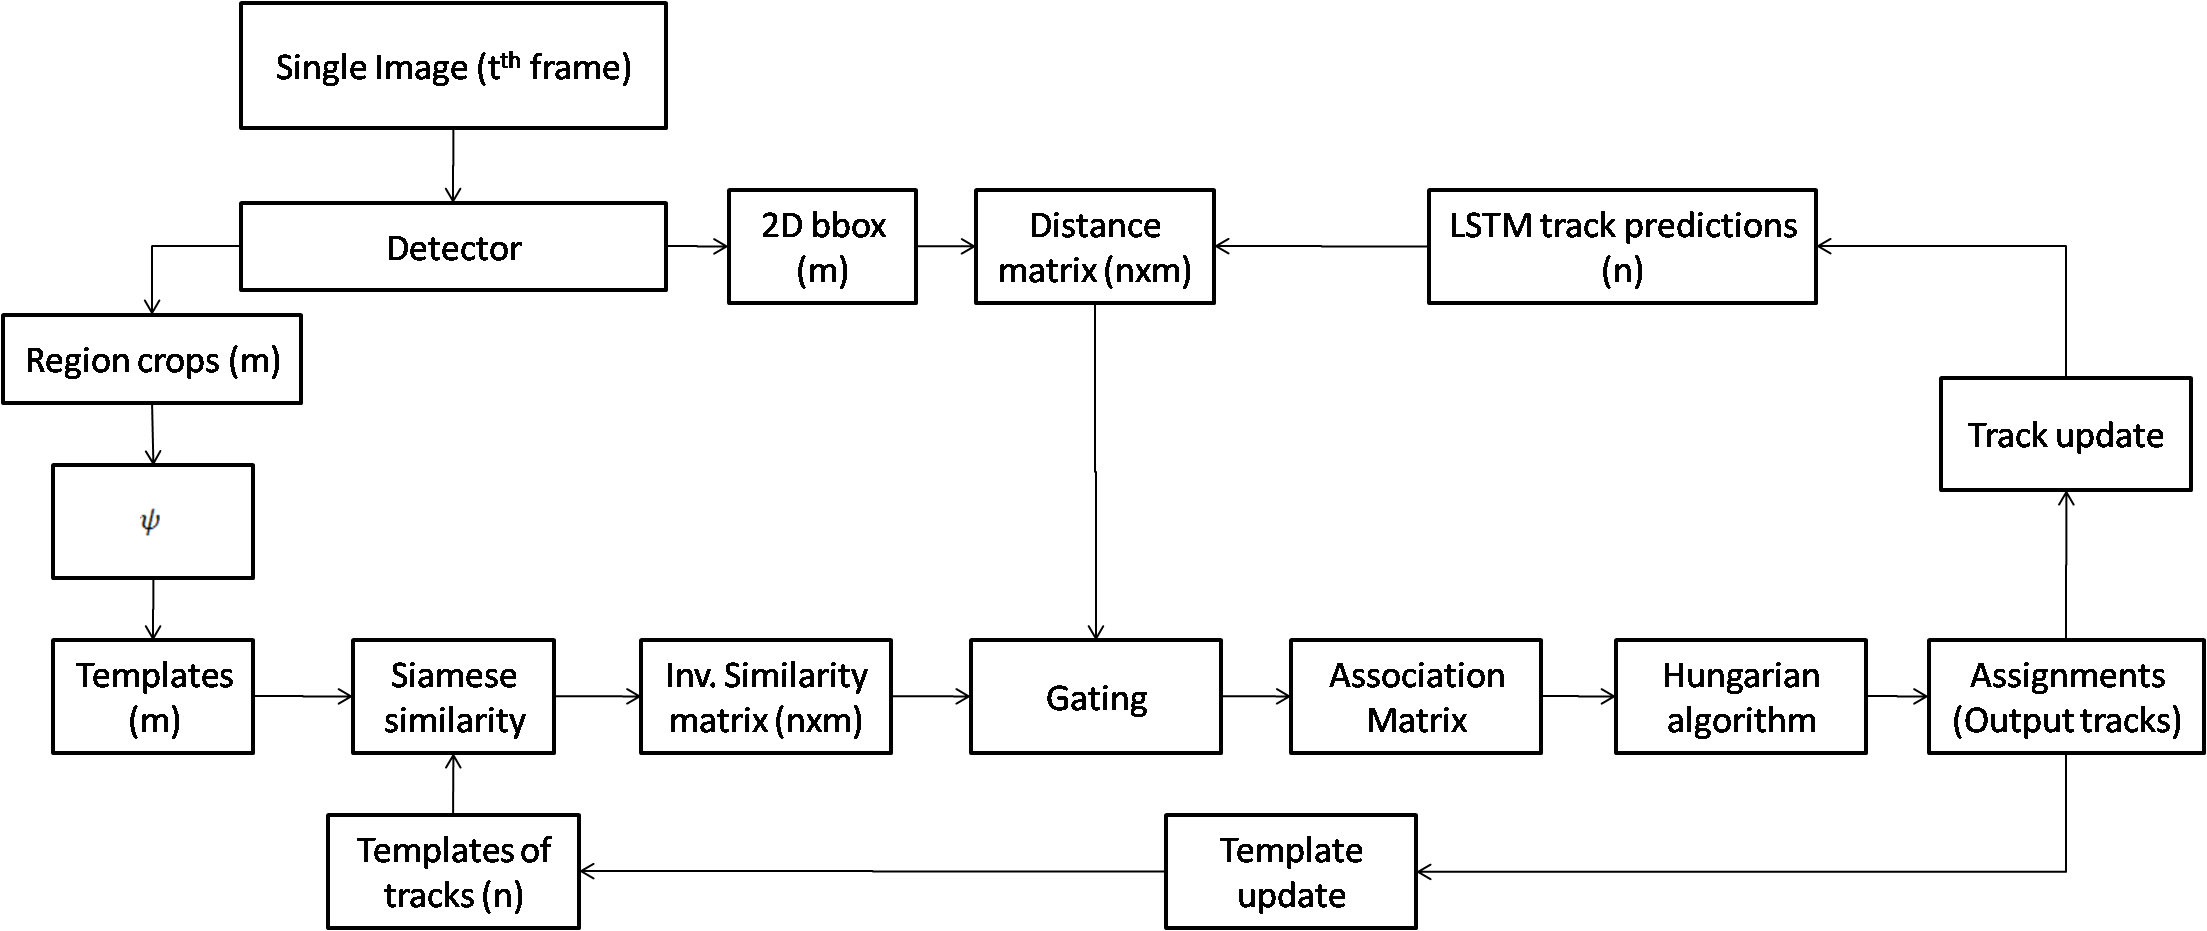
\includegraphics[ width=\textwidth]{figs/tracker.png}
	\vspace{-0.5cm}
	\caption{Overview of the overall 2D tracking system}
	\label{fig:tracker}
	\vspace{0.4cm}
\end{figure*}

\subsection{Appearance similarity}

One of the most challenging problems in this context is handling occlusions. Object tracking with the use of a Kalman filter or an LSTM network to handle spatial coherence among tracks has been a common approach. However, the uncertainty involved in the track prediction increases when tracks are exposed to prolonged occlusions. Hence it is required to re-identify occluded tracks. Deep SORT \cite{DeepSiam:deepSort} introduces the use of feature vectors to define an appearance descriptor for the purpose of track re-identification. Results presented in this work have proven this to be a successful approach. However, this comes with the additional burden of training a large network for the sole purpose of re-identification of a particular class of objects. Hence this approach is not versatile for multi-class object tracking or for online implementation. Our approach has the ability to handle multiple classes of objects and can be implemented online with ease.
\par The approach implemented in this paper involves the use of a Siamese network to determine the appearance consistency of tracks. The Siamese networks described in the SiamFC \cite{DeepSiam:SiamFC, DeepSiam:endrep} and SiamMask \cite{DeepSiam:siammask} works have proven to be highly successful in single object tracking but have not been incorporated into multi-object tracking yet. It has been trained on ImageNet datasets for similarity learning and can operate online. Thus, it can give a class independent measure for appearance consistency of tracks and therefore would be ideal for track re-identification. The network discussed in SiamFC \cite{ DeepSiam:endrep} extracts the features of the exemplar image and search image to produce a cross correlation map whose peak position corresponds to the position of the object in the exemplar image within the search image. Similarly, we use a Siamese network to produce a similarity measure between two images of the same size by building up templates through a convolution neural network (a convolution function as in \cite{ DeepSiam:endrep} shown in template generation step through  in \ref{fig:tracker})
\par The cross-correlation map produced by the Siamese network is passed through a similarity function to produce the similarity score, or more accurately an appearance cost. The similarity function in this context is defined as follows,
$$
Appearance \; Cost = A \exp(-k\sum f(x,y)) \eqno{(4)}
$$
where $f(x,y)$ is the cross correlation value at $x,y$ position in the cross correlation map and $A,k$ are tunable parameters.


\subsection{Track Association}

The track association is based on the association cost which depends on the appearance cost (from the Siamese network) as well as a distance metric. The distance metric is the measurement of how far the detection bounding box is from the bounding box of a track predicted by the LSTM. The distance metric between two bounding boxes is defined based on the IOU distance (intersection over union) between the bounding boxes. Let $ a_{i,j},c_{i,j},d_{i,j}$ represent the association cost, appearance cost and the distance metric between the $i^{th}$ detection and the $j^{th}$ track.
$$ 
a_{i,j} = 
\begin{cases} 
c_{i,j} \; if \; d_{i,j} < T \\
K \; if \; d_{i,j} \geq T \\ 
\end{cases}
\eqno{(5)}
$$
where $K$ is the gating constant and $T$ is the gating threshold. Track association is treated as an assignment problem and is carried out using the Hungarian algorithm \cite{DeepSiam:hungarian} following very closely the approach discussed in Deep SORT \cite{DeepSiam:deepSort}.

\subsection{Overall online tracking system}

The Siamese network for similarity measurement is implemented in two stages. The first stage involves producing feature maps (templates) for detections in the current frame and the next stage involves producing cross correlation maps by convolving the detection templates with track templates and generating an appearance cost matrix between track, detection pairs in that frame. These two stages have been isolated to improve the efficiency of the approach.
\par In a given frame, a crop of the bounding box corresponding to each detection is extracted. These crops are resized to 127x127 and passed through the first stage of the Siamese network to generate templates for each detection in that particular frame. These templates are passed through the second stage of the Siamese network along with the templates of tracks in order to generate a matrix of appearance costs. This cost matrix is gated according to the distance metric and subjected to the Hungarian algorithm to obtain track assignments for the detections.
\par For matched track, detection pairs; the template of the track is updated using a rolling average between the track’s current template and the template of the detection which was matched to it,
$$
temp_{track} = \gamma * temp_{track} + (1 - \gamma) * temp_{det} \eqno{(6)}
$$
where $\gamma$ is the occluded percentage of the matched detection and defined as the maximum of the Intersection over Union values (IoU) between the detection bounding boxes and the bounding box of the matched detection which is one when fully occluded and zero when the object is fully visible. Therefore, when the matched detection is fully visible, it replaces the template of the track with the template of the matched detection and when the matched detection is fully occluded, it does not update the template of the track so as not to contaminate the template with the features from occlusions.
\par Deletion of tracks and addition of new tracks is carried very similar to the approach carried out in the Deep SORT \cite{DeepSiam:deepSort} work.

\subsection{Extensibility to BEV space}
The seemingly simple but effective fact that ‘overlapping in BEV space projections cannot happen for the objects detected and predicted in 3D is exploited here through a constrained optimization problem. This work relates to the possible improvements that could be done on the system and detailed in \ref{chapter:appendix1}.

\subsection{LSTM based data association for end to end trainability}

\begin{figure*}[t]
	\centering
	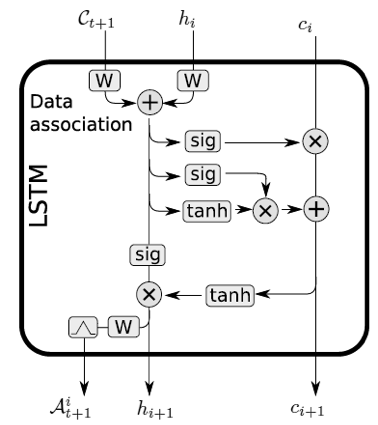
\includegraphics[width=0.5\textwidth]{figs/lstm_associate.png}
	\vspace{-0.3cm}
	\caption{Association LSTM}
	\label{fig:LSTM_network}
	\vspace{0.5cm}
\end{figure*}

The multi object tracker network uses the Hungarian algorithm for data association where this algorithm is a definite setup having an algorithmic complexity of $O(n^3)$. However the system cannot be back propagated through this implementation due to the fact that Hungarian algorithm is not differentiable. There are approaches from probabilistic view points as in \cite{russel}  and with learning perspective as presented in \cite{DeepSiam:multitarget} for obtaining a data driven system. Several experiments were conducted with data association on MOT tracking dataset based on the methodology presented in [19]. The system developed is shown in the figure below and was designed from scratch using tensorflow API. The system was designed initially to handle and check the repeated lengthy tracks in the dataset without the intervention of birth and death processes. Here the system is getting trained to build up a probability matrix $A_t$ which presents associations at time t. Thus $A_t^i=[p_{i,1},p_{i,2},p_{i,3},\ldots,p_{i,m},p_{i,m+1}]$ where  $p_{i,j}$ represents the probability of $i^{th}$  target being denoted by $j^{th}$ measurement out of m measurements for the frame (i.e. m detections).
Here 
$\sum_{j=1}^{m+1}p_{i,j}=1$ which is achieved by using softmax on the row.

The excess column presented by the last probability shows the probability that none of measurements being matched for the respective track and this track will potentially be terminated in next stages of the process.
The input $C_t\in R^{N\times M}$ is the matrix created through the second norm between the state vector $x_i$ of the target and the measurement having feature vector $z_j$.
Therefore, $C_t^{i,j}=\ xi-zj2
$

Negative log likelihood loss was used as the loss function for training. Ability to track multiple objects simultaneously in real-time and pixel-level awareness for both stuff (background) and things (objects), are two of the fundamental vision-based challenges that modern autonomous and quasi-autonomous systems are faced with. We introduce two separate novel frameworks for both problems which improve on the current state-of-the-art systems.


\section{Panoptic Segmentation}
Our work is concentrated to the assignment of a semantic label and an instance label for each pixel in an image using a novel approach of incorporating bipartite potentials to improve the segmentation accuracy.

\subsection{Background: Conditional Random Fields}

Conditional Random Fields (CRFs) are a class of statistical modeling method used for structured prediction. A CRF, used in the context of pixel-wise label prediction, models pixel labels as random variables that form a Markov Random Field (MRF) when conditioned upon the image. CRFs have primarily been used in computer vision for semantic image segmentation. In this setting, CRFs encourage the desirable properties of a good segmentation, such as the spatial consistency (e.g. spatially neighboring pixels should have the same label) and color consistency (e.g. a semantic segmentation boundary should correspond to a edge in the image) through various energy functions used in the formulation. A CRF formulation usually has energy terms arising from an imperfect classifier (sometimes known as the unary energy) and energy terms encouraging the consistency properties of the segmentation (sometimes known as the pairwise energy). Some semantic CRF models also include higher order energy terms to encourage higher order consistency properties such as consistency of the labeling within super-pixels~\cite{arnab_eccv_2016}.

Once an appropriate energy function is formed, the optimal labeling is found as the labeling that minimizes the CRF energy (or equivalently, maximizes the probability). This is known as the inference of the CRF. The exact inference of a CRF with dense pairwise connections is intractable and hence approximate inference methods such as mean field variational inference has to be utilized to solve the CRF in reasonable time~\cite{densecrf}. For a detailed treatment of CRFs, the reader is referred to~\cite{Koller_book}. 

\subsection{Bipartite CRFs}
\label{sec:body}
We propose a CRF formulation with bipartite random variables to capture interactions between semantic labels and instance labels. Inference of this CRF gives the jointly most probable semantic and instance segmentation (and therefore, the panoptic segmentation) for a given image. 

For each pixel $i$, define a pair of discrete random variables $(X_i, Z_i)$ to denote its semantic label and the instance label, respectively. For each $i$, $X_i$ can take values in $\mathcal{L} = \{l_1, l_2, \dots, l_L\}$, where each $l_j$ is a semantic label and $L$ is the number of semantic labels (includes both stuff and thing classes). Therefore, $\mathcal{L} = \Lstuff \cup \Lthings$, where $\Lstuff$ is the set of stuff class labels and $\Lthings$ the set of thing class labels. Similarly, for each $i$, $Z_i$ can take values in $\mathcal{T} = \{\inst_0, \inst_1, \dots, \inst_{\Ninst} \}$, where $\Ninst$ is the number of instances detected in the image, and the label $\inst_0$ is reserved to represent the ``no instance'' case (the pixel belongs to a stuff class).  


Let $\X = [X_1, X_2, \dots, X_N ]$ and $\Z = [Z_1, Z_2, \dots, Z_N
]$, where $N$ is the number of the pixels in the image. A joint assignment $(\x, \z)$ to these two random vectors $(\X, \Z)$ gives a unique semantic label and an instance label to each pixel $i$, and therefore represents a panoptic segmentation of the image. Note that, $\x \in \mathcal{L}^N$ and $\z \in \mathcal{T}^N$. In this work, we discuss the probability of such assignments and formulate the probability distribution function so that the ``good'' panoptic segmentation will have a high probability. We then perform inference on this formulation to find the assignment that maximizes the probability to obtain the best panoptic segmentation.

The probability of a panoptic segmentation $(\x, \z)$, given the image $I$, can be modeled as a Gibbs distribution of the following form:
\begin{equation}
\label{eqn:prob}
\Pr(\X = \x, \Z = \z|I) = \frac{1}{\mathcal{Z}(I)}\exp(-E(\x, \z|I)),
\end{equation}
where $\mathcal{Z}(I) = \sum_{(\x,\z)} \exp(-E(\x, \z|I))$, is a normalization constant, sometimes known as the partition function. The term $E(\x, \z|I)$ is known as the energy of the configuration $(\x, \z)$. Hereafter, we drop the conditioning on $I$ in the notation for brevity. The energy of our bipartite CRF is defined as follows:

\begin{equation}
\label{eqn:energy}
\begin{split}
E(\x, \z) =& \sum_i\phi(x_i) + \sum_{i < j}\Phi(x_i, x_j) \;+ \\
& \sum_i\psi(z_i) + \sum_{i < j}\Psi(z_i, z_j) \; + \\
& \sum_i\omega(x_i, z_i) + \sum_{i < j}\Omega(x_i, z_j),
\end{split}
\end{equation}
where $x_i$ and $z_i$ are the elements of the vectors $\x$ and $\z$, respectively. The meaning of each term will be described in detail below. Note that, since a ``good'' panoptic segmentation should have a high probability, it should have a low energy. Various terms in Eq.~\eqref{eqn:energy} should therefore encourage a good panoptic segmentation by penalizing disagreements with our prior knowledge about a consistent panoptic segmentation. % Roughly speaking, the energy terms represent negative log probabilities. 

\subsection{Semantic Component of the CRF}
In the following, we discuss the first two term of the energy function in Eq.~\eqref{eqn:energy}. The first term encourages the semantic segmentation result to be consistent with the initial classifier.
\begin{equation}
\phi(X_i = x_i) = - \log(\Pro(X_i = x_i)),
\end{equation}
where $\Pro(.)$ is the classifier probability score for the semantic segmentation. 

The second term in Eq.~\eqref{eqn:energy} encourages the smoothness of the semantic labeling:
\begin{equation}
\label{eq:similarity}
\Phi(X_i = x_i, X_j = x_j) = \mu(x_i, x_j) \operatorname{Sim_\Phi}(i, j),
\end{equation}
where $\mu: \mathcal{L} \times \mathcal{L} \to \mathbb{R}$ is the label compatibility function, and $\operatorname{Sim_\Phi}(i, j)$ is a similarity measure between the pixels $i$ and $j$. This term penalizes assigning different labels to a pair of pixels that are ``similar". Following \cite{densecrf}, we use a mixture of Gaussians as the similarity measure. Therefore,
\begin{equation}
\label{eqn:kernels}
\operatorname{Sim_\Phi}(i, j) = \sum_m w_{\Phi, m} \exp\left(-\frac{\|\vec{f}_i^{(m)} - \vec{f}_j^{(m)}\|^2}{2\sigma_{\Phi,m}^2}\right)
\end{equation}
where $\mathbf{f}_i$ is a feature vector for pixel $i$ containing information such as its spatial location and bilateral features (RGB + spatial coordinates). We use the same spatial and bilateral features used in~\cite{densecrf}.
\subsection{Instance Component of the CRF}

For the instance classification, we also assume the existence of an initial classifier, such as Mask R-CNN, that provides a confidence score for each instance at each pixel. Note that Mask R-CNN provides fixed-size instance segmentation predictions with respect to the bounding boxes of the detections. However, these predictions can be easily mapped to the full image by using bilinear interpolation and trivial coordinate transforms.

In the following, we use $z_i \in \{\inst_0, \inst_1, \dots, \inst_\Ninst \}$, where $\Ninst$ is the number of instances detected in the image. The label $\inst_0$ is reserved for the special case where the pixel does not belong to an instance, i.e., it belongs to a stuff class.

Similar to the semantic segmentation case, the third term in Eq.~\eqref{eqn:energy} encourages the panoptic segmentation to be consistent with the instance classifier probabilities $\Pro$:
\begin{equation}
\psi(Z_i = z_i) = - \log(\Pro(Z_i = z_i)).
\end{equation}

The fourth term in Eq.~\eqref{eqn:energy} encourages instance label consistency across the whole image by penalizing assigning different instance labels to similar pixels:
\begin{equation}
\Psi(Z_i = z_i, Z_j = z_j) = [z_i \neq z_j] \operatorname{Sim_\Psi}(i, j).
\end{equation}
The compatibility transform in this case is fixed to be $[z_i \neq z_j]$, where $[.]$ is the Iverson bracket. The similarity measure $\Sim_\Psi$ has a similar form to Eq.~\eqref{eqn:kernels}. %Intuitively, this term encourages \emph{similar} pixels to have the same instance label.

\subsection{Cross Potentials in the CRF}
An important contribution of this paper is the introduction of cross potentials between the semantic segmentation and instance segmentation. The semantic segmentation and the instance segmentation are highly related problems and therefore the solutions should agree: the semantic label at any pixel has to be compatible with the instance label at that pixel. For example, if the instance labeling says that the pixel $i$ belongs to an instance of a person class, the semantic label at pixel $i$ should also have the person label. If the initial classifier results for the instance segmentation and the semantic segmentation do not agree, one of them should correct itself depending on the interactions of other terms in the CRF.

The first cross potential term (the fifth term in Eq.~\eqref{eqn:energy}), encourages instance label and the semantic label at a given pixel to agree:
\begin{equation}
\omega(X_i = x_i, Z_i = z_i) = f(x_i, \cl(z_i)).
\end{equation}
Here, $\cl(z_i)$ is the class label of the instance $z_i$ with $\inst_0$ mapped to a special class $\operatorname{null}$. Note that, for all valid instances, the class label can be obtained from the instance classifier (e.g. Mask R-CNN). The function $f(., .): (\mathcal{L}, \Lthings \cup \{\operatorname{{null}}\}) \to \mathbb{R}^+_0$, captures the cost of incompatibility and is defined as follows: 
\begin{equation}
\label{eqn:cross_compat}
f(x_i, \cl(z_i)) = \begin{cases}
0,\;\;\text{if}\;x_i = \cl(z_i)\\
0,\;\;\text{if}\;x_i \in \mathcal{L}_{\text{stuff}}\;\text{and}\;\cl(z_i) = \operatorname{null}\\
\eta(x_i, \cl(z_i)),\;\; \text{otherwise}.
\end{cases}
\end{equation}
The above function covers three cases: 1) If the semantic label and the class label of the instance label match, there will be no penalty for such assignment since there is no incompatibility in this case. 2) If the semantic segmentation assigns a stuff label and the instance segmentation assigns $\inst_0$ label, there will be no penalty in that case either. 3) If the semantic label and the instance label mismatch, there will be a penalty with the magnitude decided by the function $\eta(., .): \Lthings \cup \{\operatorname{null}\} \times \Lthings \cup \{\operatorname{null}\} \to \mathbb{R}^+$. This function is learned from data as described in Section~\ref{sec:infer}.

The last term in Eq.~\eqref{eqn:energy}, encourages the consistency of semantic label and the instance label among similar looking pixels and has the form:
\begin{equation}
\Omega(X_i = x_i, Z_j = z_j) = f(x_i, \cl(z_j))\; \operatorname{Sim_\Omega}(i, j),
\end{equation}
where each symbol has the meaning described above.


\subsection{Inference and Parameter Optimization}
\label{sec:infer}
The best panoptic segmentation given the model described in Section~\ref{sec:body} is the assignment $(\x, \z)$ that maximizes the probability in Eq.~\eqref{eqn:prob}. However, since the graphical model used in BCRF has dense connections between the pixels, the exact inference is infeasible. We therefore use an approximate parallel mean field inference algorithm following~\cite{densecrf}.

In this setting, the joint probability distribution is approximated by the product of marginal distributions:
\begin{equation}
\label{eq:q_approx}
\Pr(\X=\x, \Z=\z) \approx \prod_i Q_i(x_i)\,R_i(z_i),
\end{equation}
where $Q_i(x_i) = \Pr(X_i = x_i)$ and $R_i(z_i) = \Pr(Z_i = z_i)$ are the marginal distributions. Out of all the distributions that can be written down in this factorized form, the closest distribution to the original joint distribution is found by minimizing the KL divergence~\cite{Koller_book, densecrf}. For our BCRF formulation, this results in the iterative algorithm detailed in Algorithm~\ref{alg:infer}.

To make our model flexible, we deliberately include a number of parameters in the BCRF model, which we automatically learn from the training data. More specifically, the BCRF model has the following parameters:
\begin{enumerate}
	\item Weight multipliers for different energy terms: each term in Eq.~\eqref{eqn:energy} is multiplied with a weight parameter, which decides the relative strength of the term. This parameterization helps learn the optimal combination of different energies in the CRF. For example, if the initial semantic segmentation model has better accuracy than the instance segmentation model, the $\phi$ unary energy might be weighted more than the $\psi$ unary energy.
	
	\item Parameters for similarity functions: Each similarity function $\Sim_X(i, j)$ of the form shown in Eq.~\eqref{eq:similarity} has its own parameters. These learn the relative strength of spatial and appearance consistency of the panoptic segmentation.
	
	\item Label compatibility matrices: The two functions $\mu(., .)$ and $\eta(., .)$ are initialized to have a zero cost for a pair identical labels and a fixed cost for any combination of two different labels. They are then given the freedom to automatically learn the relative penalty strengths for different label combinations.
\end{enumerate}


\subsection{BCRF in a Deep Network}
In this section, we discuss how BCRF can be used in a deep network. In~\cite{Zhen_ICCV15_CRFRNN}, authors showed that, in the semantic segmentation setting, mean field inference of a CRF with Gaussian pairwise potentials can be formulated as a Recurrent Neural Network (RNN). Since our BCRF also uses an iterative mean field algorithm of similar nature, it is readily adaptable into the RNN based inference described in~\cite{Zhen_ICCV15_CRFRNN}. Therefore, BCRF can be a first-class citizen of a deep network performing panoptic segmentation. Importantly, this formulation allows automatic optimization of the BCRF parameters described in Section~\ref{sec:infer}, using backpropagation and a gradient descent algorithm such as stochastic gradient descent (SGD). This is a major advantage since it allows us to increase the number of parameters used in BCRF, and hence increase its flexibility, without adding to the burden of manual parameter optimization.

In the current state-of-the-art methods, semantic segmentation and instance segmentation are solved with different network architectures with complimentary strengths. The BCRF formulation given a systematic way of combining these strengths in a probabilistic framework. Such an example usage of BCRF is shown in Figure~\ref{fig:bcrf_net}. The CNN feature extractor here can be a common backbone network such as ResNet-101 or ResNeXt. The semantic segmentation branch is usually a fully convolutional network that is capable of seeing a wide field of view, whereas the instance segmentation branch is a region-proposal based network such as Mask R-CNN. The semantic segmentation branch's output is taken as the $\phi$ unary potential input to the BCRF, and instance segmentation branch's output as the $\psi$ unary potentials. In addition, the raw image is also fed into the BCRF to derive the similarity functions $\Sim_X(., .)$ using the pixel locations and the RGB values. 

During the training of the network, in the forward pass, BCRF inference is performed using Algorithm~\ref{alg:infer}. A suitable loss function for panoptic segmentation can then be used at the output of the network. In the backward pass, differentials with respect to the loss function will be passed into the BCRF inference to optimize various parameters used in the BCRF model. Importantly, during the backward pass, after BCRF inference, the error differentials can be passed on to the semantic branch and the instance branch both to optimize their parameters, and subsequently, the feature extractor CNN's parameters. Therefore, the whole network, including the BCRF component, can be jointly trained.


